% !TeX spellcheck = de_DE
\documentclass[10pt,a4paper]{article}
\usepackage{fontspec}
%\usepackage[utf8]{inputenc}
\usepackage{amsmath}
\usepackage{amsfonts}
\usepackage{amssymb}
\usepackage{mathrsfs}
\usepackage{graphicx}
\usepackage[ngerman]{babel}
\usepackage{listings}
\usepackage{color}
\usepackage{subcaption}
\usepackage{mathtools}


\definecolor{Brown}{cmyk}{0,0.81,1,0.60}
\definecolor{OliveGreen}{cmyk}{0.64,0,0.95,0.40}
\definecolor{CadetBlue}{cmyk}{0.62,0.57,0.23,0}
\definecolor{lightlightgray}{gray}{0.95}
\definecolor{mediumgray}{gray}{0.65}
\definecolor{darkgray}{gray}{0.3}
\definecolor{MatlabKeyWordBlue}{cmyk}{0.92,0.92,0,0}
\definecolor{MatlabKeyWordBlue}{rgb}{0.13,0.13,1}
\definecolor{MatlabCommentGreen}{rgb}{0.1529,0.6029,0.1529}
\definecolor{MatlabStringPurple}{rgb}{0.62,0.12,0.94}
%\definecolor{MatlabCommentGreen}{cmyk}{0.75,0,0.75,0.45}
\definecolor{cadmiumorange}{rgb}{0.93, 0.53, 0.18}
\definecolor{darkorange}{rgb}{1.0, 0.55, 0.0}
\definecolor{bluekeywords}{rgb}{0.13,0.13,1}
\definecolor{greencomments}{rgb}{0,0.5,0}
\definecolor{redstrings}{rgb}{0.85,0,0}
\definecolor{pycharmString}{rgb}{0.64,0.760,0.38}





\lstdefinestyle{myMatlabStyle}{
	language=matlab,                        % Code langugage
	basicstyle=\ttfamily,                   % Code font, Examples: \footnotesize, \ttfamily
	keywordstyle={\color{bluekeywords}\bfseries}, % Keywords font ('*' = uppercase)
	commentstyle={\color{greencomments}\bfseries},% Comments font
	stringstyle=\color{MatlabStringPurple},  % String font
	numbers=left,                           % Line nums position
	numberstyle=\tiny,                      % Line-numbers fonts
	stepnumber=1,                           % Step between two line-numbers
	numbersep=5pt,                          % How far are line-numbers from code
	backgroundcolor=\color{lightlightgray}, % Choose background color
	frame=none,                             % A frame around the code
	tabsize=2,                              % Default tab size
	captionpos=b,                           % Caption-position = bottom
	breaklines=true,                        % Automatic line breaking?
	breakatwhitespace=false,                % Automatic breaks only at whitespace?
	showspaces=false,                       % Dont make spaces visible
	showstringspaces=false,
	showtabs=false,                         % Dont make tabls visible
	morekeywords={try, catch},  			% CUDA specific keywords
}

\title{
	{\huge TU WIEN} \\
	{\Large \textbf{Einführung in die Methode der finiten Elemente}} \\
	{\large Mathematik Fachvertiefung}}
%\author{Benjamin Kulnik}
\author{
	\\
	von \\
	\\
	\textit{Benjamin Kulnik} \\
	1425900 \\
	benjamin.kulnik@student.tuwien.ac.at \\
}






\begin{document}
	\begin{titlepage}
		\centering
		\maketitle
		%{benjamin.kulnik@student.tuwien.ac.at\par}
		%{1425900\par}
		\vfill
		
	\end{titlepage}
	\tableofcontents
	
	% !TeX spellcheck = de_DE
\section{Finite Differenzen Methode}
	Als Beispiel sei das elektrische Skalarpotential $V$ eines Zylinderkondensators zu bestimmen, also das Lösen der Differentialgleichung:
	\begin{equation}
	-\frac{1}{r} \frac{\partial}{\partial r} ( r \frac{\partial }{\partial r} u(r)) = 0
	\end{equation}
	was dem elektrischen Skalarpotential entspricht.
	\begin{equation}
		\vec \nabla \cdot \epsilon_0 \vec \nabla V = 0
		\label{e-potential}
	\end{equation}
	Aufgrund der Symmetrie - es wird passenderweise ein Zylinderkoordinatensystem gewählt - kann das Problem eindimensional betrachtet werden, also:
	\begin{equation}
	V(r,\phi, z) = V(r)
	\end{equation}
	Als Randbedingung sind $V(r=1)=0$ und $V(r=5)=100$ vorgegeben. 
	\\
	
	{\Large Aufgaben \par}
	\begin{enumerate}
		\item Bestimmen Sie die analytische Lösung $u(r)$.
		\item Bestimmen Sie eine numerische Lösung mittels Methode der finiten Differenzen indem Sie das Intervall (1,5) gleichmäßig in 4 Teilintervalle teilen und den Differentialoperator diskretisieren.
		\item  Vergleichen Sie die analytische Lösung mit der numerischen Lösung. Wie groß ist der relative Fehler in \% in den Knotenpunkten?
	\end{enumerate}
	
	
	\subsection{Analytische Lösung}
	Die Differentialgleichung kann analytisch gelöst werden. Hierzu wird zuerst das erste Differenzial aufgelöst und die Gleichung auf folgende Form gebracht:
	\begin{equation}
	\frac{1}{r} \frac{\partial }{\partial r} u(r) +  \frac{\partial^2}{\partial r^2} u(r) = 0
	\end{equation}
	umformen und integrieren:
	\begin{eqnarray}
		-\frac{1}{r} \frac{\partial}{\partial r} ( r \frac{\partial }{\partial r} u(r)) = 0 \\
		 \frac{\partial}{\partial r} ( r \frac{\partial }{\partial r} u(r)) = 0 \\
		  r \frac{\partial }{\partial r} u(r) = C_1 \\
		  \frac{\partial }{\partial r} u(r) = \frac{C_1}{r} \\
	\end{eqnarray}
	
%	Wir wissen, wie die Lösung ungefähr auszusehen hat, nämlich in etwa die Form $u=C r^\lambda$ haben wird. Wir können also also diesen allgemeinen Ansatz wählen und in die Gleichung einsetzen (dabei wurden die konstanten Faktoren gleich gekürzt).
%	Das führt dann auf:
%	\begin{equation}
%	\lambda \frac{1}{r} r^{\lambda-1} + \lambda^2 r^{\lambda -2} = 0
%	\end{equation}
%	Wie leicht zu erkennen ist, können auch die $r$'s gekürzt werden und anschließend $\lambda$ bestimmt werden. Mit
%	\[
%	\lambda_1 = 0 , \quad \lambda_2 = -1
%	\]	
%	erhalten wir nun als allgemeine Lösung unserer homogenen Differentialgleichung
%	\begin{equation}
%	u(r) = C_1 r^{\lambda_1} + C_2 r^{\lambda_2} = C_1 + C_2 \frac{1}{r}
%	\end{equation}
%	mit noch zu bestimmenden Konstanten $C_1$ und $C_2$. Diese werden so gewählt, dass die Lösung unsere Randbedingungen erfüllt. Für $u(1) = 0$ ergibt sich:
%	\begin{equation}
%	u(1)=C_1 + C_2 = 0 \quad \Rightarrow \quad C_1 = - C_2
%	\end{equation}
%	Und für die zweite Randbedingung ergibt sich (für $C_2$ wurde gleich $-C_1$ eingesetzt):
%	\begin{equation}
%	u(5)=C_1 - C_1 \frac{1}{5} = 100 \quad \Rightarrow \quad C_1 = -125
%	\end{equation}
	
	Nochmaliges integrieren nach $r$ bringt uns schließlich auf
	\begin{equation}
	u(r)= 	\int \frac{\partial u}{\partial r} dr = C_1 \ln r + C_2
	\end{equation}
	mit noch zu bestimmenden Konstanten $C_1$ und $C_2$. Diese werden so gewählt, dass die Lösung unsere Randbedingungen erfüllt. Für $u(1) = 0$ ergibt sich:
	\begin{equation}
	u(1)=C_1 \ln(1) + C_2 =  0 \quad \Rightarrow \quad C_2 = 0
	\end{equation}
	Und für die zweite Randbedingung ergibt sich:
	\begin{equation}
	u(5)=C_1 \ln(5)  = 100 \quad \Rightarrow \quad C_1 =\frac{100}{\ln 5} \approx 62.13349...
	\end{equation}
	\\
	

	
	\subsection{Numerische Lösung}
	Für die nummerische Berechnung wurde das Intervall in 4 Teilintervalle aufgeteilt und jeweils das Potential an den Stützstellen $r=\{1,2,3,4,5\}$ berechnet.	Die Gleichung \ref{e-potential} ist ausgeschrieben und in Zylinderkoordinaten:
	\begin{equation}
	-\frac{1}{r} \frac{\partial}{\partial r} ( r \frac{\partial }{\partial r} u(r)) = 0
	\end{equation}
	Durch Anwenden der Produktregel lässt sich das Gleichgungssystem auf 
	\begin{equation}
	\frac{1}{r} \frac{\partial}{\partial r} ( r \frac{\partial }{\partial r} u(r)) = \frac{1}{r} \frac{\partial }{\partial r} u(r) +  \frac{\partial^2}{\partial r^2} u(r) = 0
	\end{equation}
	Da wir $u(r=1)=0$ und $u(r=5)=100$ bereits kennen, konstruieren wir einen Vektor mit den gesuchten Werten der Knotenpunkte $2,3,4$:
	\begin{equation}
	\mathbf{u} =	\begin{bmatrix}
	u_2\\
	u_3\\
	u_4
	\end{bmatrix}
	\end{equation}
	Das Differential wird numerisch mit dem zentralen Differenzen Quotient angenähert:
	\begin{equation}
	\frac{\partial u(r)}{\partial r} \approx \frac{u(r+h)-u(r-h)}{2 h}
	\end{equation}
	und entsprechend für die zweite Ableitung wurde
	\begin{equation}
		\frac{\partial^2 u(r)}{\partial r^2} \approx \frac{u(r+h)-2u(r)+u(r-h)}{h^2}
	\end{equation}
	gewählt. Die Herleitung erfolgt über die Taylorreihen-Entwicklung.
	
	Wir konstruieren unser lineares Gleichungssystem folgendermaßen:
	\begin{equation}
	\frac{1}{2rh} \mathbf{A} \mathbf{u} + \frac{1}{h^2}\mathbf{B}  \mathbf{u} = \mathbf{f}
	\end{equation}
	wobei die Matrizen $\mathbf{A}$ und $\mathbf{B}$ die Koeffizienten für die Differnezenquotienten enthalten. Der Vektor $\mathbf{f}$ enthält die rechte Seite der Differenzialgleichung (die hier allerdings immer 0 ist) und außerdem die entsprechenden Randbedingungen die zum Lösen erforderlich sind.
	\begin{equation}
	\mathbf{f} = \begin{bmatrix}
	\frac{1}{rh} u_1  - \frac{1}{h^2} u_1 \\
	0 \\
	-\frac{1}{2rh} u_5  - \frac{1}{h^2} u_5 
	\end{bmatrix}
	\end{equation}
	Ausgeschrieben erhält man mit $h=1$ und $r=\{2,3,4\}$:
	\begin{equation}
	\frac{1}{2}
	\begin{bmatrix}
	0 & \frac{1}{2} & 0 \\ 
	-\frac{1}{3} & 0 & \frac{1}{3} \\ 
	0 & -\frac{1}{4} & 0
	\end{bmatrix}   
	\begin{bmatrix}
	u_2\\
	u_3\\
	u_4
	\end{bmatrix} +   \begin{bmatrix}
	-2 & 1 & 0 \\ 
	1 & -2 & 1 \\ 
	0 & 1 & -2
	\end{bmatrix}  \begin{bmatrix}
	u_2\\
	u_3\\
	u_4
	\end{bmatrix} = \begin{bmatrix}
	\frac{1}{2} u_1  -  u_1 \\
	0 \\
	-\frac{1}{8} u_5  -  u_5 
	\end{bmatrix}
	\end{equation}
	Die Matrizen können leicht zusammengefasst werden und anschließend gelöst werden.


	\subsection{Implementierung in Matlab}
	\lstinputlisting[language=matlab,style=myMatlabStyle,caption={Implementierung der FDM für die Berechnung des Potenzials in einem Zylinderkondensators. Eine Anpassung der Anzahl der Stützstellen ist möglich über die Variable $N$}]{../Matlab/FDM.m}
	
	\subsection{Ergebnisse}
	
	Die Methode der finiten Differenzen erlaubt eine zuverlässige Berechnung einer einfachen Differentialgleichung. Der relative Fehler ist selbst bei wenigen Stützstellen sehr gering.
		
	\begin{figure}[!h]
		\centering
	\begin{tabular}{cc}
		\begin{subfigure}{0.45\linewidth}
			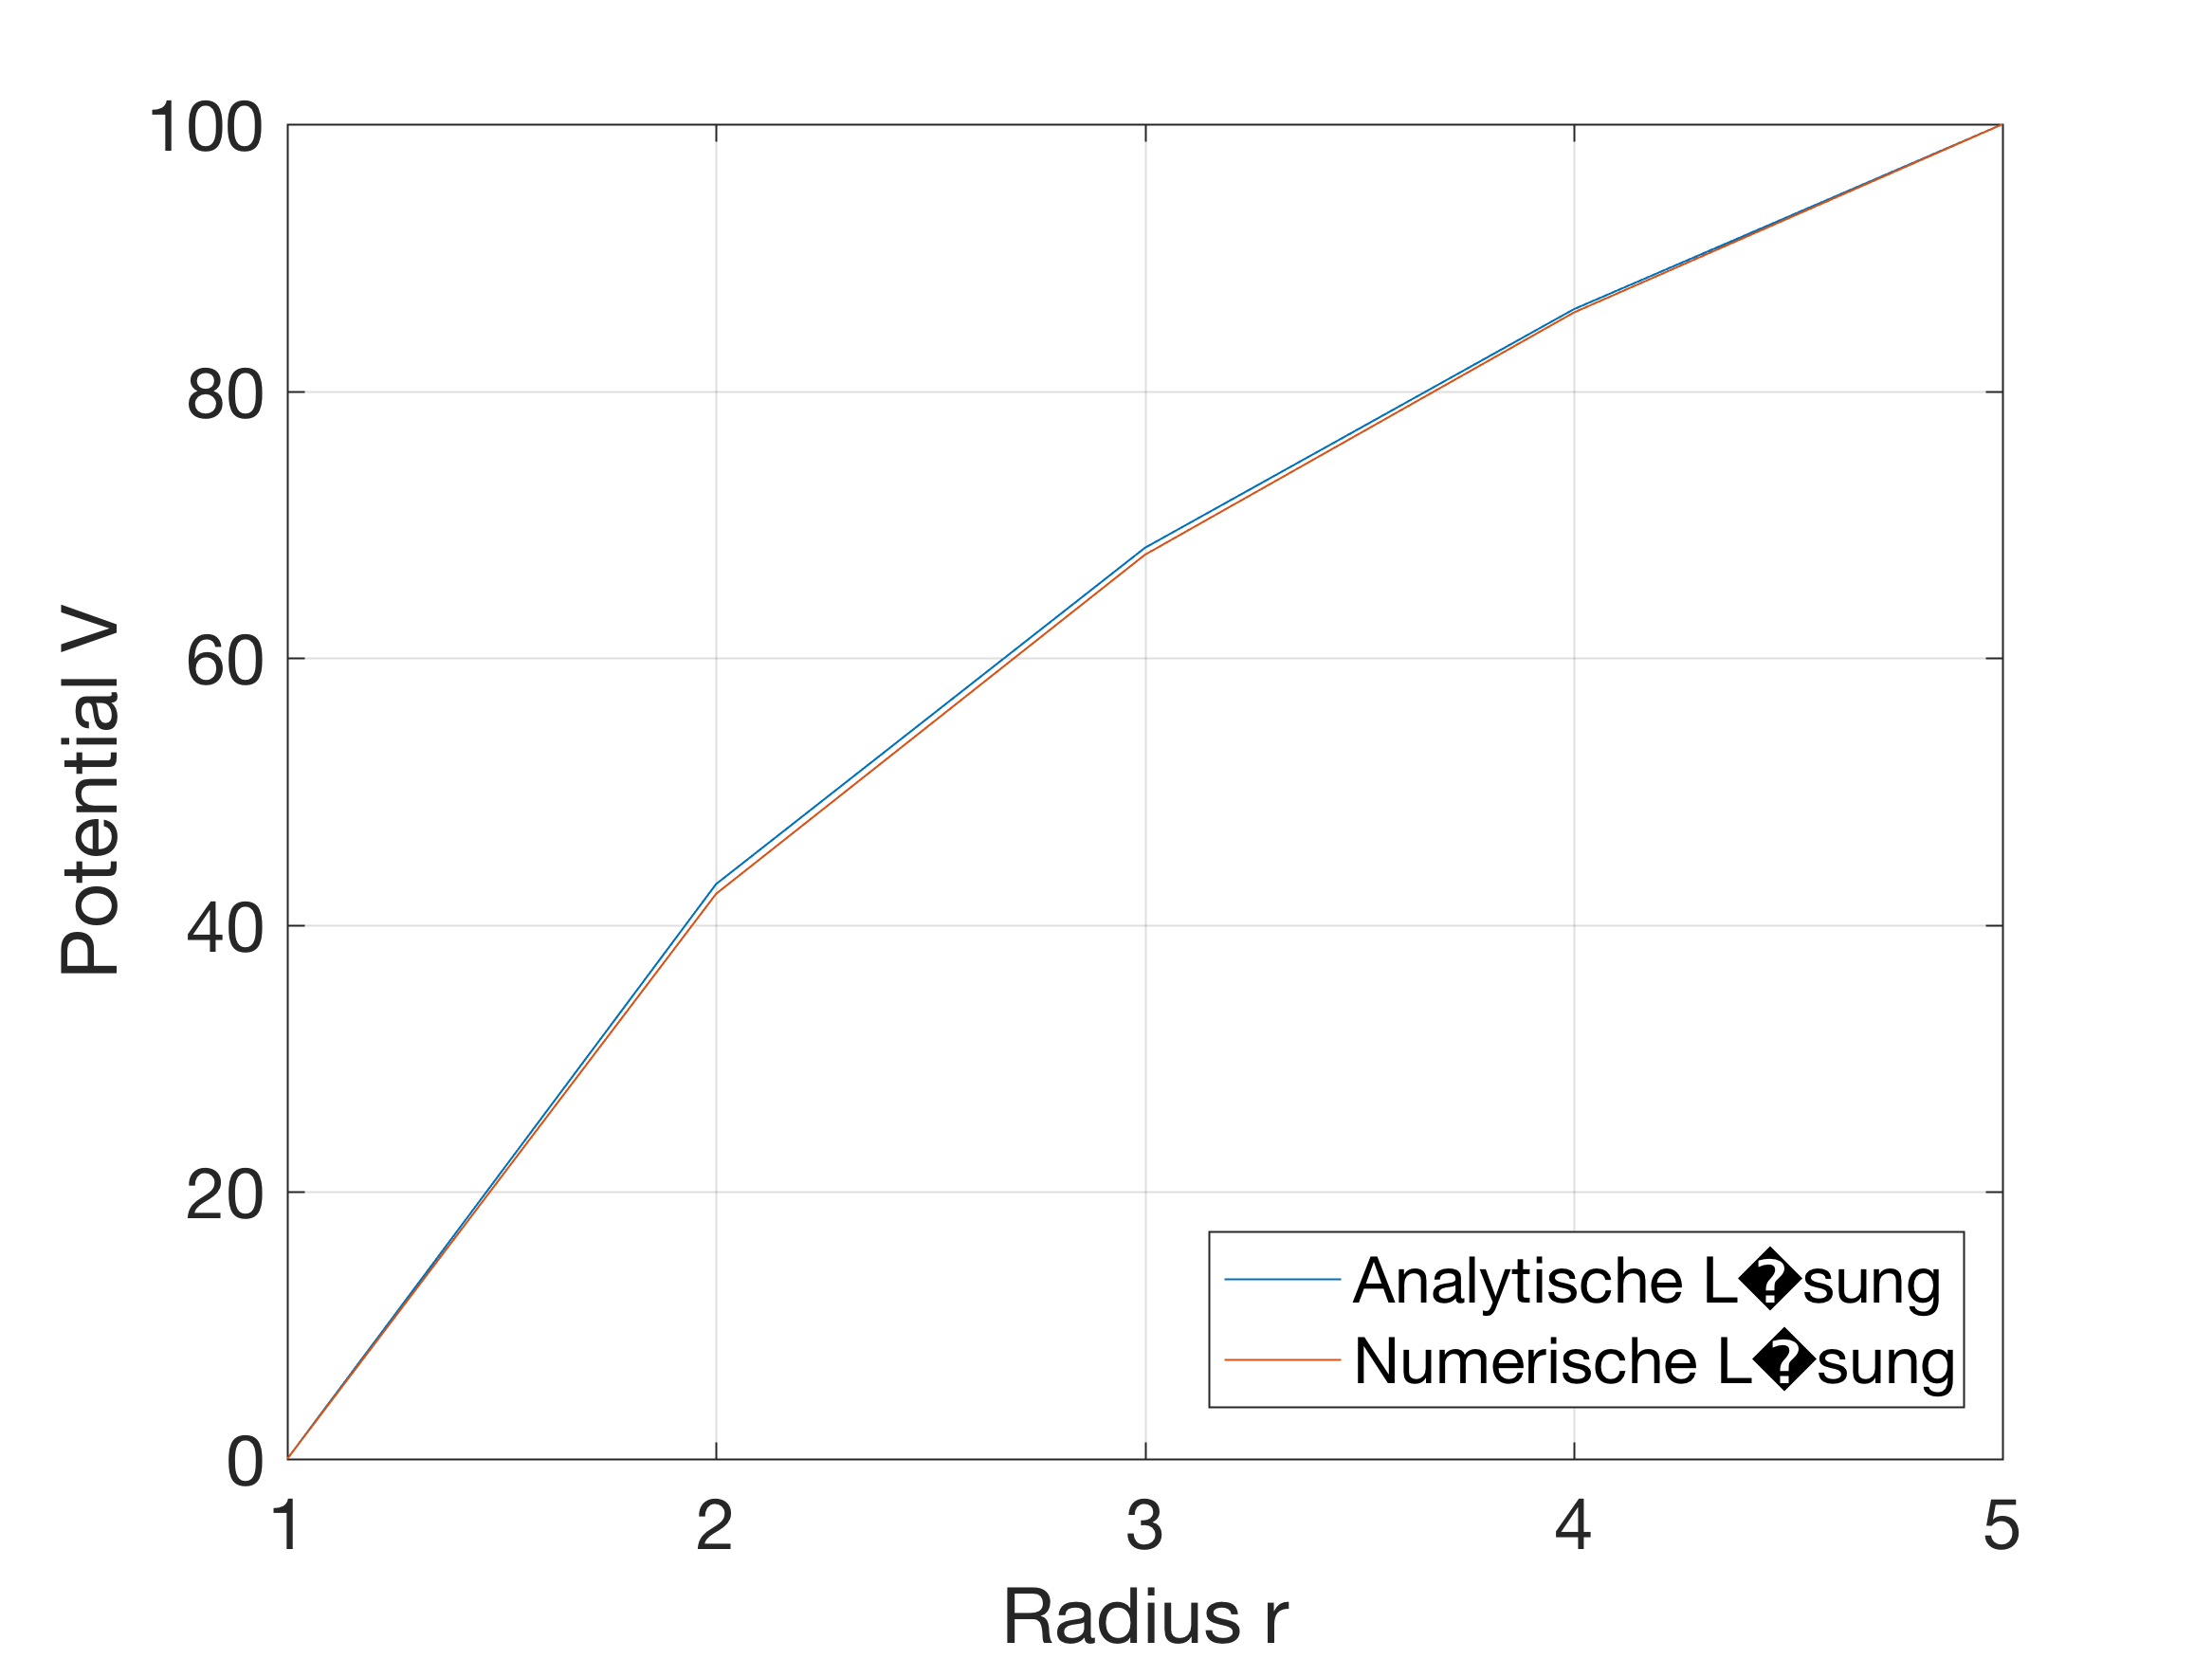
\includegraphics[width=\linewidth]{../Matlab/cylinder}
			\caption{Plot}
			\label{fig:cylinder}
		\end{subfigure}
		~
		\begin{subfigure}{0.45\linewidth}
			
			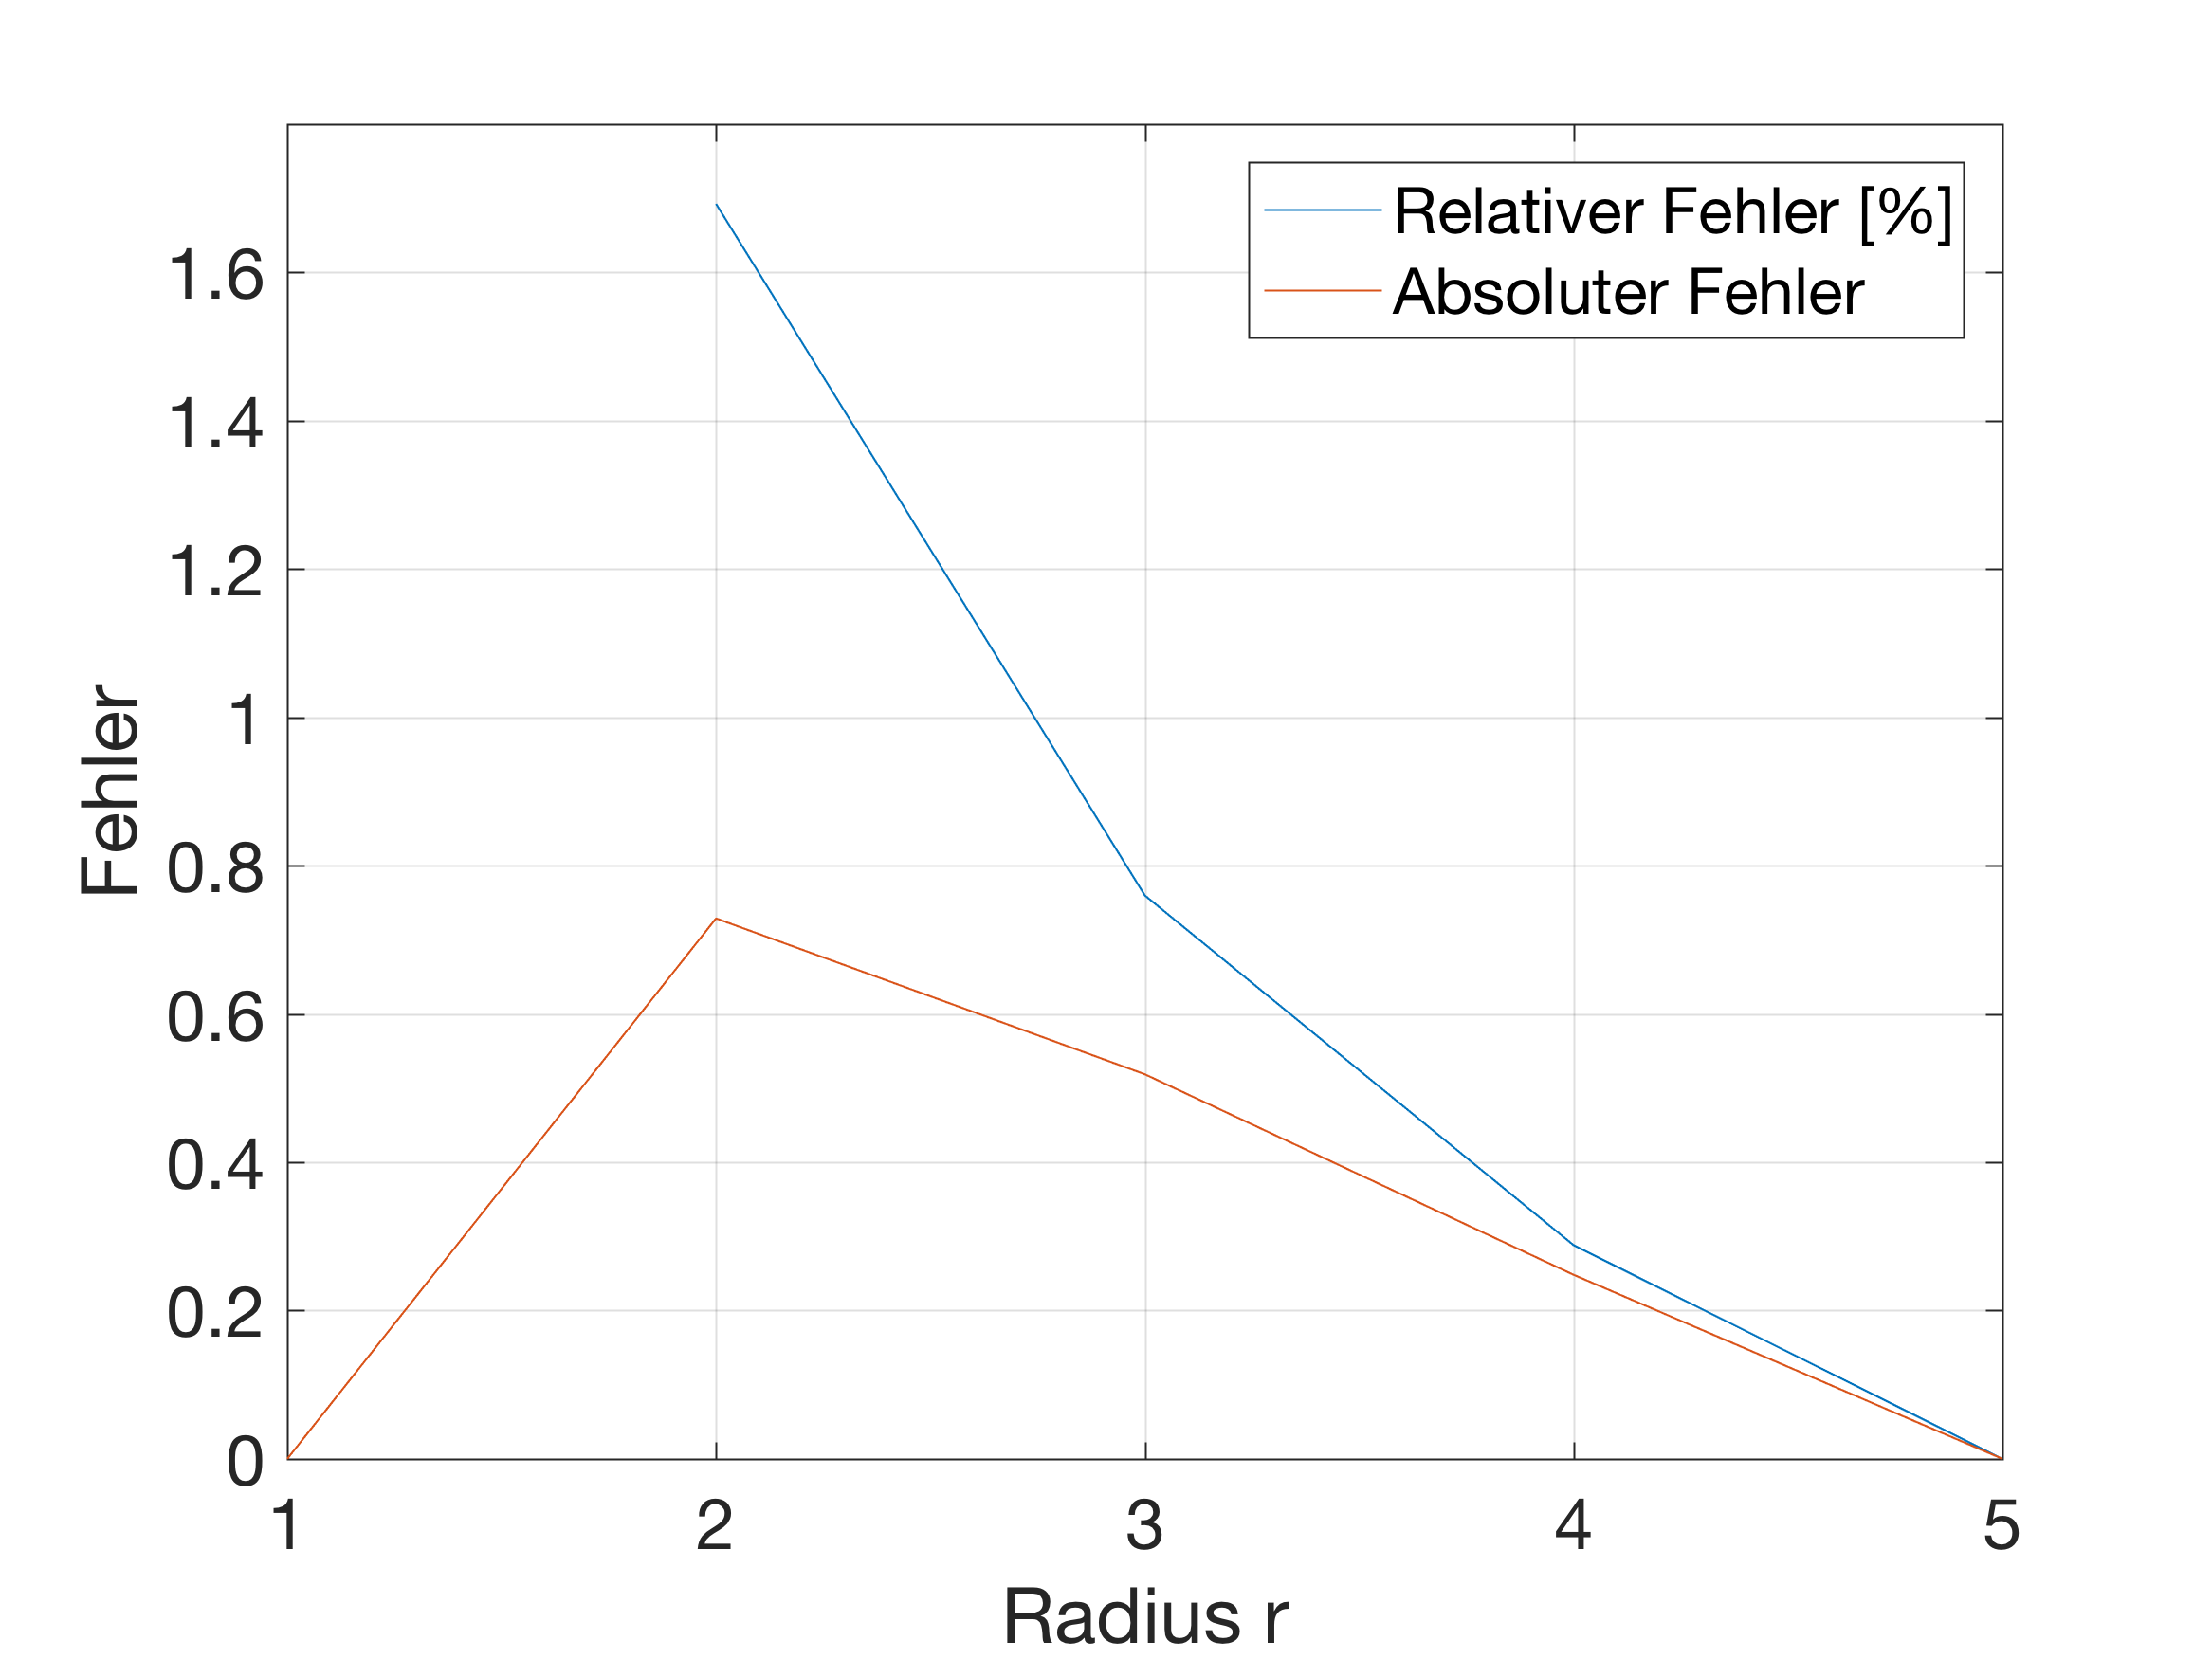
\includegraphics[width=\linewidth]{../Matlab/error}
			\caption{Error}
			\label{fig:error}
		\end{subfigure}
		
	\end{tabular}
	\caption{Ergebnisse für 3 Stützstellen im Intervall $r=[1,5]$}
	\end{figure}

	\begin{table}[!h]
	\centering
	\caption{Ergebnisse der FDM für $N=3$}
	\begin{tabular}{|c|c|c|c|}
		\hline 
		&  Analytisch & Numerisch & Relativer Fehler [\%] \\ 
		\hline 
		$u_2$ & 43.0677 & 42.3387 & 1.6926 \\ 
		\hline 
		$u_3$ & 68.2606 & 67.7419 & 0.7599 \\ 
		\hline 
		$u_4$ & 86.1353 & 85.8871 & 0.2882 \\ 
		\hline 
	\end{tabular} 

  



	
	\end{table}
	% !TeX spellcheck = de_DE
\section{Finite Elemente Methode}
	
	\subsection{Angabe}
	Es soll die Methode der finiten Elemente (FEM) auf folgende Gleichung angewendet werden.
	\begin{equation}
		\frac{\partial^2 u(x,t)}{\partial ^2 x} - \mu_0 \epsilon_0 \frac{\partial ^2 u (x,t)}{\partial^2 t} = 0
	\end{equation}
	Mit den Randbedingungen
	\begin{align}
	u(a,t) &= 0 \\
	- \frac{\partial}{\partial x} u(b,t)+\sqrt{\mu_0 \epsilon_0} \frac{\partial}{\partial t} u(b,t) &= 0
	\end{align}
	Mit den Anfangsbedingungen
	\begin{align}
	u(x,0) &= w(x) = e^{-k(2x-a-b)^2} \\
	\frac{\partial}{\partial t} u(x,0) &= 0
	\end{align}
	soll das Newmarksche Zeitschrittverfahren durchgef�hrt werden.
	\\
	
	{\Large Aufgaben \par}
	\begin{enumerate}
		\item Leiten Sie dazu die schwache Formulierung f�r die Abh�ngigkeit vom Ort her.
		\item Nehmen Sie eine geeignete L�nge des Intervalls $[a, b]$ an und unterteilen Sie es gleichm��ig in $n$ finite Elemente der L�nge $h$.
		\item Verwenden Sie Hutfunktionen als Basisfunktionen. Ber�cksichtigen Sie die Randbedingungen und erstellen Sie die Steifigkeitsmarix $\mathbf{S}_h$ und die Massenmatrix $\mathbf{M}_h$.
		\item L�sen Sie das gew�hnliche Differentialgleichungssystem
	\[
	\mathbf{S}_h \mathbf{u}_h  + \mathbf{M}_h \frac{\partial ^2}{\partial t^2} \mathbf{u}_h = \mathbf{0}
	\]
		mit dem Newmark-Zeitschritt-Verfahren
	\end{enumerate}


	
	\subsection{Herleiten der schwachen Formulierung}
	\subsubsection{Allgemeine Idee}
	Wir betrachten Differentialgleichungssysteme auf einem Gebiet $\Omega$ (etwa ein Teil der reellen Zahlen $\mathbb{R}$) mit vorgegeben Werten (Randbedingungen) an $\partial \Omega$ die sich der Art 
	\begin{equation}
		\mathbf{A}\mathbf{u}=\mathbf{f}
	\end{equation}
	anschreiben lassen. Dabei ist $\mathbf{u}$ die gesuchte Funktion. Alle Faktoren und Differentialoperatoren werden durch $\mathbf{A}$ ausgedr�ckt. 
	Die Idee ist nun u durch eine Ansatzfunktion $u_h$ zu approximieren.
	Diese Ansatzfunktion soll in etwa die Gestalt einer Summe von (Laplace'schen) Ansatzfunktion multipliziert mit einem Tr�gerfunktion $p_i(x)$ sein. Diese Tr�gerfunktion soll im gesamten Gebiet mit Ausnahme eines kleinen Bereichs (eines \textit{Tr�gers}) verschwinden, also konstant 0 sein. Dadurch teilt man 
	\begin{equation}
		u_h = \sum_{i=0}^N u_i p_i(x)
	\end{equation}
	Diese Ansatzfunktion ver�ndert unsere Funktion $u$, deshalb wird sie im Allgemeinen die Gleichung \textbf{nicht} erf�llen. Der linke Teil der Gleichung minus dem rechten Teil wird nicht exakt 0 sondern ein gewissen Wert $r$ ergeben. Dieser Fehler $r(x)$ wird \textit{Residuum} gennant.
	\begin{equation}
	\mathbf{r} =\mathbf{f}-\mathbf{A}\mathbf{u}_h \neq 0 \tag{allgemein}
	\end{equation}
	und in unserem Beispiel
	\begin{equation}
		r(x) =\frac{\partial^2 u_h(x,t)}{\partial ^2 x} - \mu_0 \epsilon_0 \frac{\partial ^2 u_h (x,t)}{\partial^2 t} \neq 0 
	\end{equation}
	Der tats�chliche Fehler (also der Differenz  $e=u-u_h$) kann, im Gegensatz zum Residuum, nicht bestimmt werden, da die Funktion $u$ nicht bekannt ist. Das Residuum kann jedoch bestimmt werden und dieses gilt es zu minimieren. Gesucht ist nun also:
	\begin{equation}
		\min{\mathbf{r}} = \min{\mathbf{f}-\mathbf{A}\mathbf{u}_h} =  0  \tag{hoffentlich}
	\end{equation}
	Bisher war es die Aufgabe die Funktion $u_h$ zu finden ($A$ und $f$ sind ja bekannt), welche die Residuuen verschwinden l�sst. Wenn $u_h$
	Dazu w�hlen wir f�r die schwache Formulierung eine bekannte Gewichtsfunktion $w(x)$ und multiplizieren damit unsere Gleichung (\textit{Methode der gewichteten Residuuen}). Anschlie�end integrieren wir �ber das gesamte Gebiet $\Omega$ (was in unserem eindimensionalen Fall dem Intervall $[a,b]$ entspricht). Damit ergibt sich: 
	\begin{align}
	\int_{\Omega} r(x)w(x) dx = 0 \\
	\int_{a}^{b} u_h''(x,t) w(x) dx - \mu_0 \epsilon_0 \int_{a}^{b}\frac{\partial ^2 }{\partial t^2}u_h (x,t)w(x) dx =0 
	\label{weak-form}
	\end{align}
	Mit der verallgemeinerten Ableitung der Distributionen in $H$ (dem Sobolev-Raum, welcher Funktionen, f�r die eine verallgemeinerte Ableitung existiert umfasst):
	\begin{equation}
		\int_{a}^{b} u_h''(x) w(x) dx = -\int_{a}^{b} u_h'(x) w'(x) dx + u_h'(x)w(x) \vert_a^b 
		\label{distribution-differential}
	\end{equation}
	An $x=a$ (allgemeiner $\Gamma_D = \{a\}$) liegt eine Dirichlet'sche Randbedingung vor, was so viel bedeutet wie das $u(a,t)=\text{const}$ ist, damit muss die Weg-Ableitung $u'(a,t)$ verschwinden. Generell gilt hier, dass durch das Einsetzen der Ansatzfunktionen N Gleichungen erzeugt werden. Da der wert von $u$ an der Stelle $\Gamma_D = \{a\}$ allerdings bereits bekannt ist, wird diese Gleichung nicht ben�tigt damit kann $w(a)=0$ gew�hlt werden. Au�erdem ist in unserem konkreten Fall noch eine Cauchy'sche Randbedingung an $\Gamma_C = \{b\}$ vorgegeben: 
	\[u'(b,t)=u_x(b,t) = \sqrt{\mu_0 \epsilon_0} u_t(b,t) ~~~~ \forall t \in  [0,t_0]\] daraus folgt also
	\begin{equation}
		u'(x,t)w(x) \vert_a^b = \sqrt{\mu_0 \epsilon_0} u_t (b,t) w(b) - \underbrace{u'(a,t)w(a)}_{=0}
	\end{equation}
	
	\subsection{Festlegen des Intervalls}
	Bei der Methode der finiten Elemente wird eine stetige Funktion auf $N$ Teilintervalle (Elemente) zerlegt. Dazu werden Funktionswerte an Knotenpunkten berechnet und diese mit auf kleine Intervalle beschr�nkten Funktionen multipliziert. F�r das Intervall $x = \{a,...,b\}$ kann die Zerlegung folgenderma�en aussehen:
	\begin{equation}
	x_i = a + i h
	\end{equation}
	wobei die Schrittweite $h=\frac{b-a}{N}$ ist. Im Prinzip kann diese Zerlegung aber beliebig gew�hlt werden.
	\subsection{Ansatzfunktion}
	F�r die Funktion $u$ wird eine Interpolation $u_h$ folgender Gestalt gew�hlt:
	\begin{equation}
	u \approx u_h = \sum_{i = 0}^{N} u_i  p_i(x)
	\end{equation}
	Dies entspricht einer Summe von Ansatzfunktion gewichtet mit noch zu bestimmenden konstanten Faktoren $u_i$. Diese Ansatzfunktion k�nnen verschiedene Gestalten haben, sollten jedoch die Eigenschaft aufweisen einen kompakten Tr�ger zu besitzen, d.h. $p_i(x) = 0$ f�r alle $x > a+ih$ und $x < a-ih$. Zwischen zwei Knotenpunkten ist der Wert der Funktion nicht bekannt und muss entsprechend interpoliert werden und da sich zwischen den Kontenpunkten mehrere Ansatzfunktionen i.A. �berlagern, sollte darauf geachtet werden, dass die Summe immer gleich 1 ist, also
	\begin{equation}
	p(x) = \sum_{i=0}^{N} p_i(x) = 1 ~~\forall x \in [a,b] 
	\end{equation} 
	Da die Koeffizienten $u_i$ nun konstante Faktoren sind, wird die (Weg-)Ableitung auf $p(x)$) �bertragen. Das bedeutet:
	\begin{equation}
	u_h'(x,t) = \sum_{i = 0}^{N} u_i  p_i'(x)
	\end{equation}
%	Setzen wir dies in die allgemeine Formel \ref{generic-linear-equation} ein, erhalten wir:
%	\begin{equation}
%	A(\sum_{i = 0}^{N} u_i  p_i(x))-f(x,t)  \overset{!}{=} 
%	 0
%	\end{equation}
	In diesem Beispiel wird als Ansatzfunktionen verschobene Dreckeisfunktionen ('Hutfunktionen') verwendet. Selbstverst�ndlich muss bei der Auswahl darauf geachtet werden, dass die gew�hlte Ansatzfunktion hinreichend oft differenzierbar ist.

	\begin{figure}
		\centering
		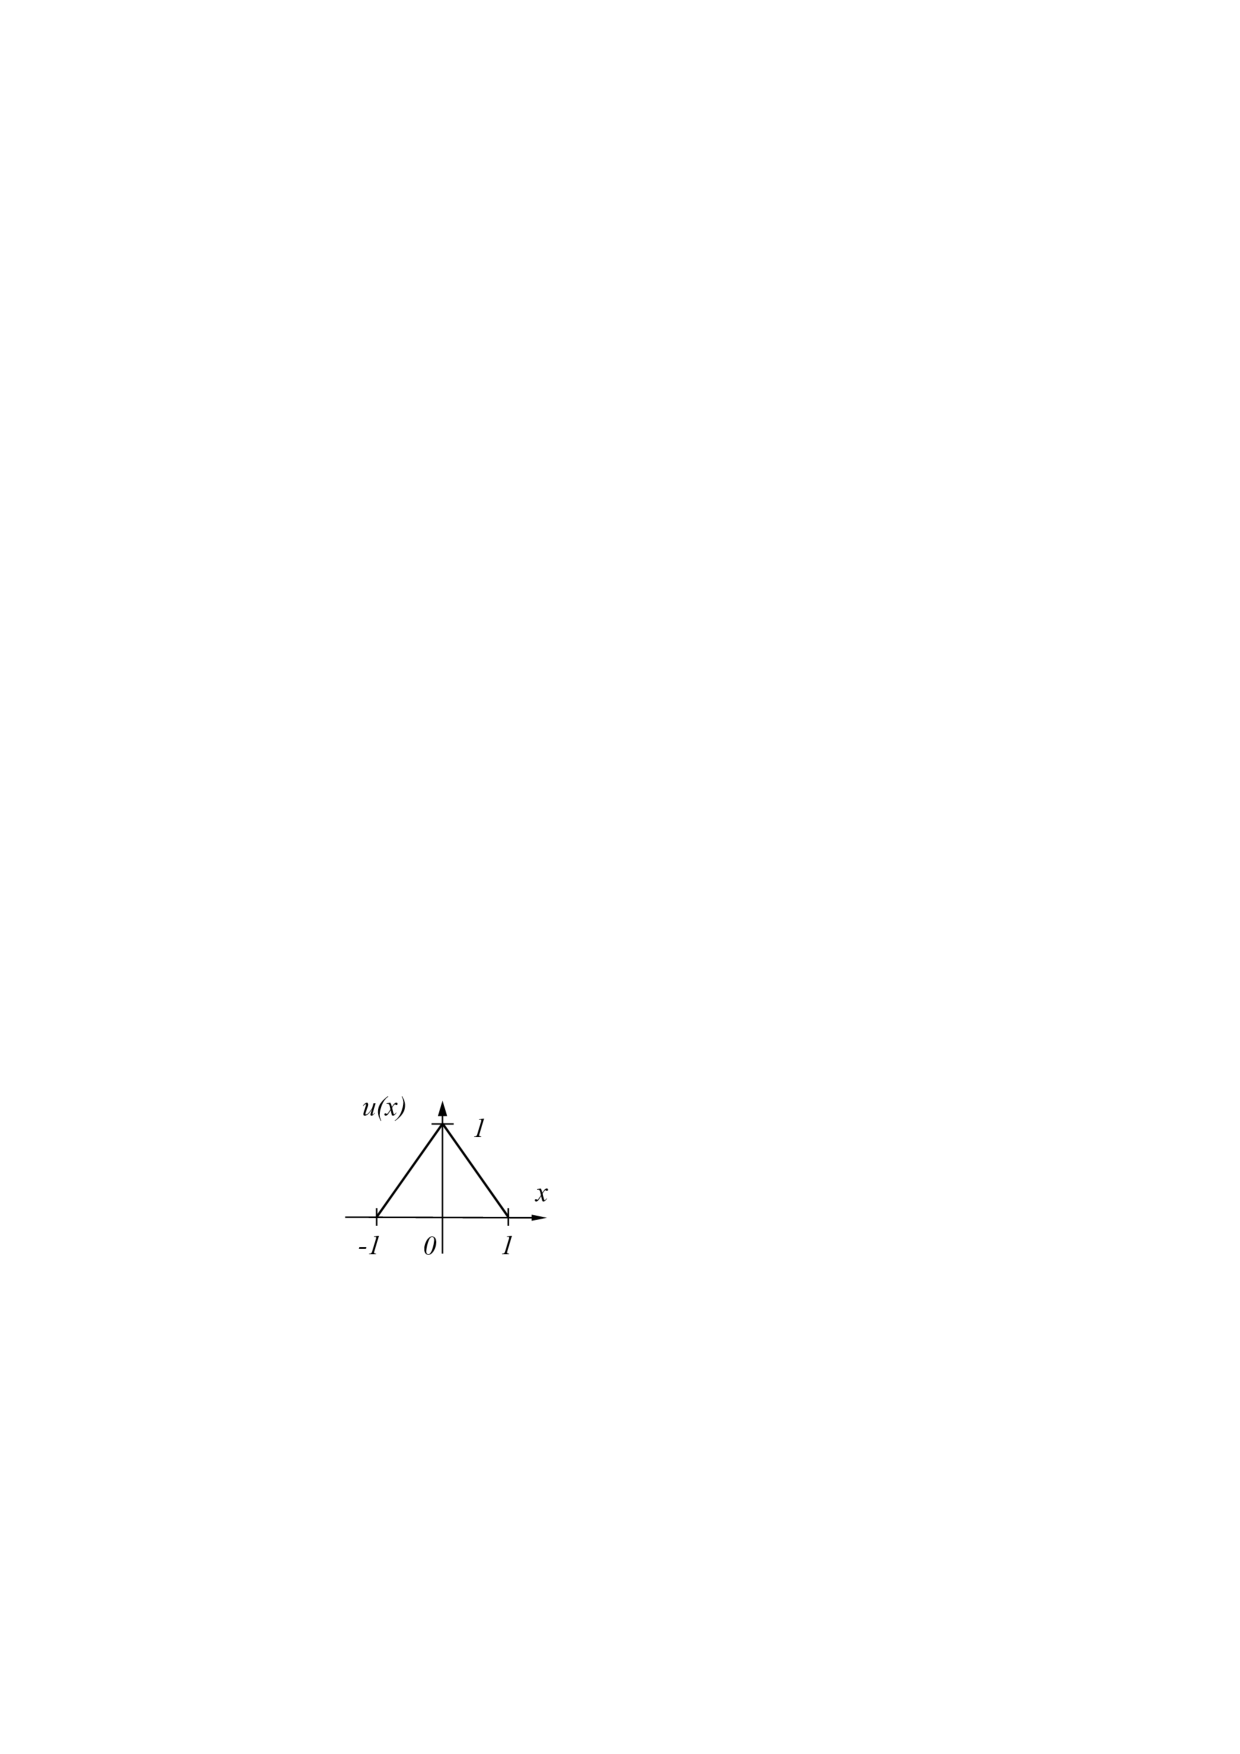
\includegraphics[width=0.5\linewidth]{img/hut}
		\caption[Hutfunktion]{Hutfunktion}
		\label{fig:hut}
	\end{figure}


	
	Setzen wir dies nun in die Herleitung der schwachen Formulierung \ref{weak-form} ein, erhalten wir mit etwas umformen und unter Verwendung der verallgemeinerten Ableitung aus Formel \ref{distribution-differential}. Da sich unser Intervall zeitlich nicht �ndert, darf die Zeit-Ableitung vor das Integral gezogen werden.
	\begin{equation}
	\sum_{i = 0}^{N} u_i   \int_{a}^{b} p_i'(x) w'(x) dx - 
	\mu_0 \epsilon_0 \frac{\partial ^2 }{\partial t^2} \sum_{i = 0}^{N} u_i \int_{a}^{b}p_i(x)w(x) dx = 0
	\label{weak-form2}
	\end{equation}
	Hier gelten noch $u_1,u_2,...u_N$, also $N$ Unbekannte Koeffizienten, zu finden. F�r $N$ unbekannte Koeffizienten werden bekanntlich $N$ unabh�ngige Gleichungen ben�tigt. Ein Weg diese zu erhalten ist �ber die Ansatzfunktion $v(x)$. F�r diese Ansatzfunktion wird ebenfalls eine �hnliche Zerlegung wie f�r $p(x)$ festgelegt, sollte es sogar die selbe sein, handelt es sich um die \textit{Galerkin Methode}. Man setzt also
	\begin{equation}
	w(x) = p(x) = \sum_{j = 0}^{N} p_j(x)
	\end{equation}
	und setzt dies dann in die Gleichung (\ref{weak-form2}) ein.
	\begin{equation}
	\sum_{i = 0}^{N} u_i \sum_{j = 0}^{N}\int_{a}^{b} p_i' p_j' dx 
	+ 
	\sqrt{\mu \epsilon} \frac{\partial}{\partial t} u_i \sum_{j = 0}^{N} p_i(B) p_j
	= 
	\mu \epsilon \sum_{i = 0}^{N} \frac{\partial ^2 }{\partial t^2} u_i 
	\sum_{j = 0}^{N} \int_{a}^{b} p_i p_j dx
	\end{equation}
	
	Da wir Hutfunktionen verwenden k�nnen, welche durch die Dreiecksfunktion $p_i = tri(\frac{x + ih}{h})$ beschrieben werden, k�nnen die Integrale gel�st werden:
	
	\begin{equation}
	\int_{a}^{b} p_ip_j dx = \begin{cases}
	\frac{4}{6}h, ~~ j=i \\
	\frac{1}{6}h,~~ j=\{i-1,i+1\}\\
	0\, ~~\text{sonst}
	\end{cases}
	\end{equation}
	und f�r $p'_i p'_j$ gilt
	\begin{equation}
	\int_{a}^{b} p_i' p_j' dx = \begin{cases}
	\frac{2}{h}, ~~ j=i \\
	-\frac{1}{h},~~ j=\{i-1,i+1\}\\
	0\, ~~\text{sonst}
	\end{cases}
	\end{equation}
	Ausgenommen sind hier die Ergebnisse die direkt am Rand liegen. Bei $\Gamma_D = \{a\}$ ist der Wert von $u$ bereits bekannt, die Ansatzfunktion kann also ohne weiteres Null gesetzt werden. Bei $\Gamma_C = \{b\}$ ist nur der Wert der Ableitung von $u$ bekannt. Hier muss der Wert erst bestimmt werden. Bei Betrachtung der Situation am Rand sieht man, dass hier nur �ber die \textit{halbe} Ansatzfunktion integriert wird, also das auch genau halb so gro� ist.
	\begin{figure}
		\centering
		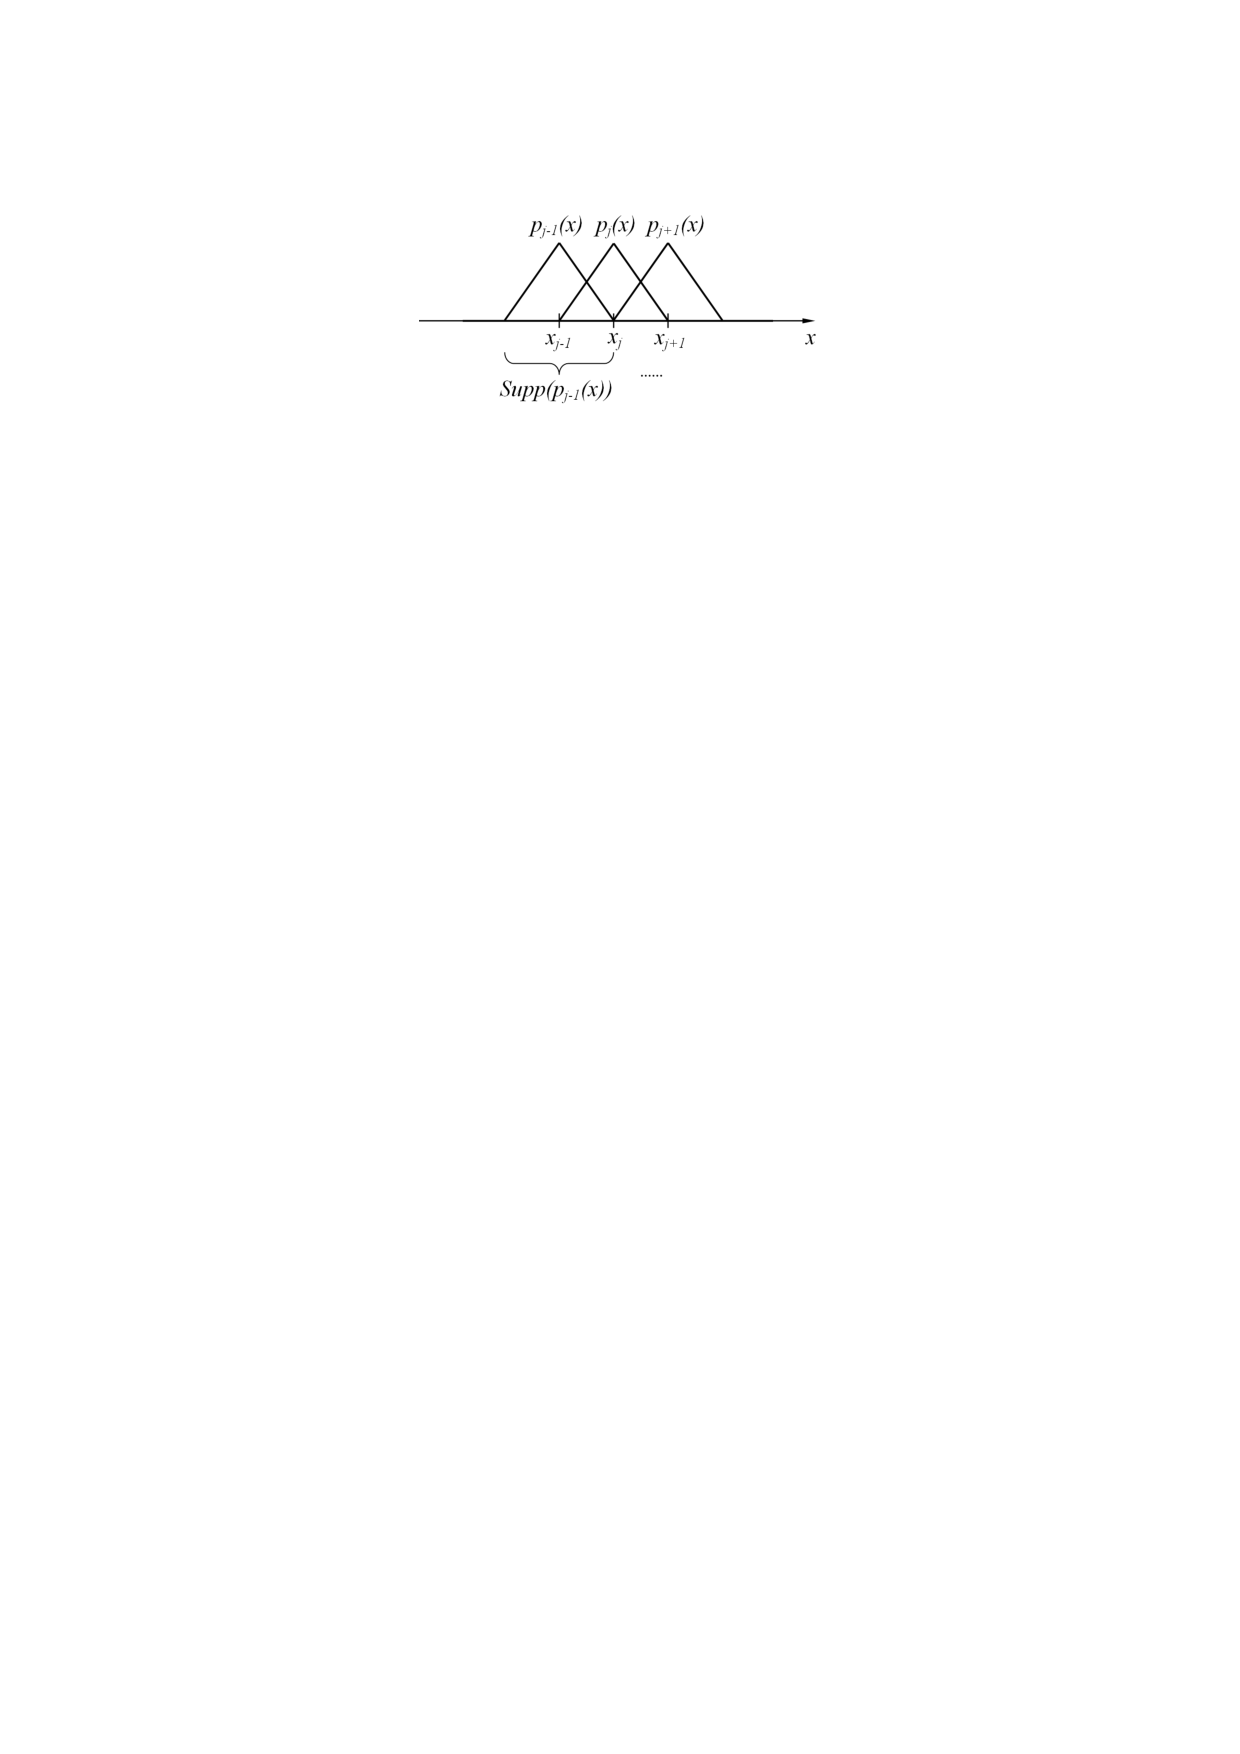
\includegraphics[width=0.7\linewidth]{img/hutfunktionen}
		\caption{�berlagerte Hutfunktionen}
		\label{fig:hutfunktionen}
	\end{figure}
	
	Damit kann das Gleichungssystem in der Form
	
	\begin{equation}
	\mathbf{S}_h \mathbf{u}_h + \mathbf{C}_h \frac{\partial}{\partial t} \mathbf{u}_h + \mathbf{M}_h \frac{\partial ^2}{\partial t^2} \mathbf{u}_h = \mathbf{0}
	\end{equation}
	
	folgenderma�en angeschrieben werden:
	
	\begin{align}
	\begin{split}
	\frac{1}{h}   
	&\begin{bmatrix}
	2 & -1 & 0 & \cdots & 0 \\ 
	-1 & 2 & -1 & \cdots & 0 \\ 
	0 & -1 & 2 & \ddots & \vdots \\ 
	\vdots & \vdots & \ddots & \ddots & -1 \\ 
	0 & 0 & \cdots & -1 & 1
	\end{bmatrix} 
	\begin{bmatrix}
	u_1 \\ 
	u_2 \\ 
	\vdots \\ 
	u_N
	\end{bmatrix}  +
	\\
	+
	\sqrt{\mu_0 \epsilon_0} 
	&\begin{bmatrix}
	0 & 0 & 0 & \cdots & 0 \\ 
	0 & 0 & 0 & \cdots & 0 \\ 
	0 & 0 & 0 & \ddots & \vdots \\ 
	\vdots & \vdots & \ddots & \ddots & 0 \\ 
	0 & 0 & \cdots & 0 & 1
	\end{bmatrix} 
	\frac{\partial}{\partial t} 
	\begin{bmatrix}
	u_1 \\ 
	u_2 \\ 
	\vdots \\ 
	u_N
	\end{bmatrix}
	+ \\ +
	\mu_0 \epsilon_0 \frac{h}{6}
	&\begin{bmatrix}
	4 & 1 & 0 & \cdots & 0 \\ 
	1 & 4 & 1 & \cdots & 0 \\ 
	0 & 1 & 4 & \ddots & \vdots \\ 
	\vdots & \vdots & \ddots & \ddots & 1 \\ 
	0 & 0 & \cdots & 1 & 2
	\end{bmatrix} 
	\frac{\partial ^2}{\partial t^2} 
	\begin{bmatrix}
	u_1 \\ 
	u_2 \\ 
	\vdots \\ 
	u_N
	\end{bmatrix} = 
	\begin{bmatrix}
	0 \\ 
	0 \\ 
	\vdots \\ 
	0
	\end{bmatrix}
	\end{split}
	\end{align}
	
	\subsection{Newmark Zeitschrittverfahren}
	
	Hier werden die partiellen Zeitableitung durch die Variablen $u, v, a$ dargestellt.
	\[
	u = u(t_j) , \quad 
	\frac{\partial u}{\partial t} \approx v(t_j) , \quad
	\frac{\partial^2 u}{\partial t^2} \approx a (t_j)
	\]
	Diese sind eine Anlehnung an die Mechanik, wo die erste Ableitung des Weges nach der Zeit die Geschwindigkeit $v$, und die zweite Ableitung nach der Zeit die Beschleunigung $a$ bezeichnet.
	Das Newmark-Verfahren beruht auf einer Taylor-Entwicklung f�r $u$ und $v$, wobei
zweite Ableitungen durch Beschleunigungen zum Zeitpunkt $t_j$ und $t_{j+1}$ approximiert werden. F�r den Zeitpunkt $t_{j+1} = tj + \Delta t$ ergibt sich das Gleichungssystem
	
	\begin{equation}
	\mathbf{Su}_{j+1} + 	\mathbf{Cv}_{j+1} +	\mathbf{Ma}_{j+1} = 	\mathbf{f}_{j+1}
	\label{eq:newmark}
	\end{equation}
	
	\begin{align}
		v_{j+1} &= v_j + \Delta t  [(\frac{1}{2}-\gamma)a_j + \gamma a_{j+1}] \\
		u_{j+1} &= u_j + \Delta t v_j + \frac{(\Delta t)^2}{2} [(\frac{1}{2}-\beta)a_j + \beta a_{j+1}]
	\end{align}
	
	mit $\beta = \frac{1}{4}$ und $\gamma = \frac{1}{2}$.
	
	Die Gleichung \ref{eq:newmark} kann auf einen der drei Parameter umgeformt werden und es ergibt sich
	\begin{equation}
	(\mathbf{S} + \gamma \Delta t	\mathbf{C} +	\mathbf{M})a_{j+1} = 	\mathbf{\tilde f}_{j+1}
	\label{eq:newmark-final}
	\end{equation}
	wobei die Gr��en $u_j$, $v_j$ und $a_j$ in den Vektor $\mathbf{\tilde f}_{j+1}$ sind. Herleitung siehe Skriptum.
	
	
	\subsection{Implementierung in Matlab}
	\lstinputlisting[language=matlab,style=myMatlabStyle,caption={Implementierung der FEM f�r ein eindimensionales L�sen der Wellengleichung}]{../Matlab/FEM.m}	
	
	
	\subsection{Ergebnis}
	
	Die Methode der finiten Elemente in Kombination mit dem Newmark'schen Zeitschrittverfahren bringt sehr brauchbare Ergebnisse hervor. Jedoch neigt das Verfahren, trotz einhalten der Stabilit�tsbedingung nach ausreichend vielen Zeitschritten
	\begin{equation}
		\Delta t < \frac{\Delta x^2}{v}
	\end{equation}
	 zur Instabilit�t.
	
	\begin{figure}[!h]
		\centering
		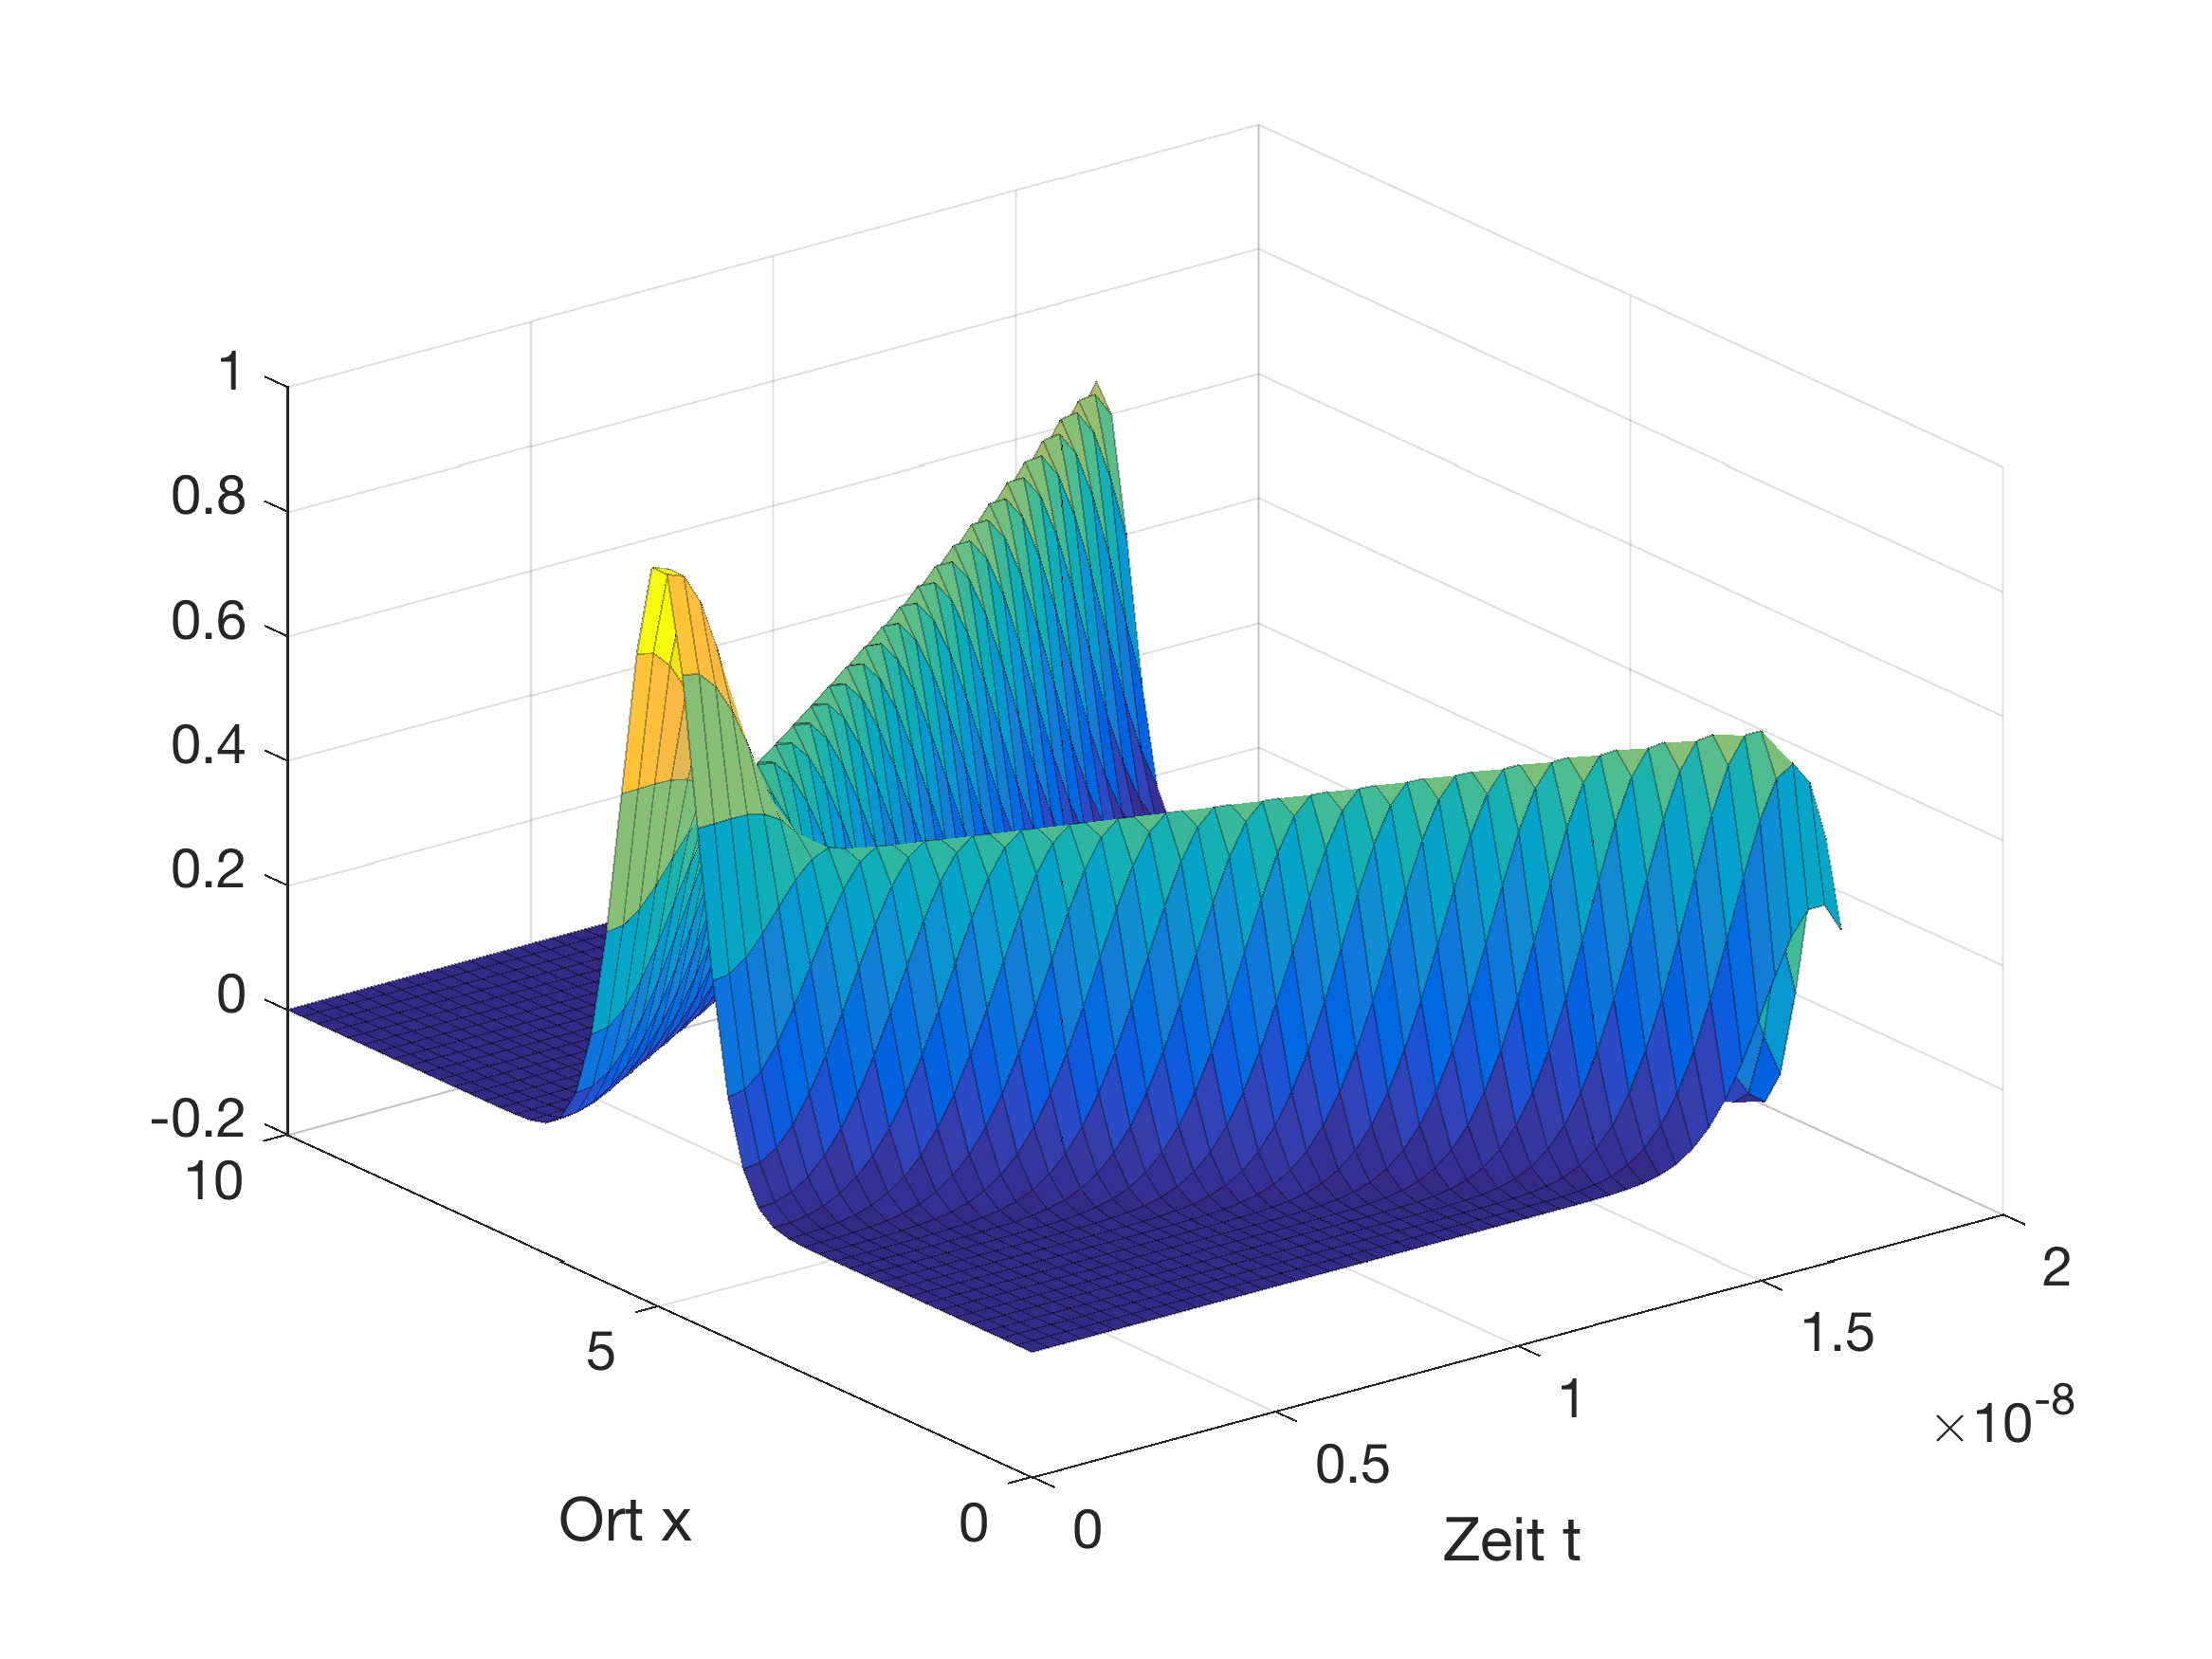
\includegraphics[width=\linewidth]{../Matlab/wave}
		\caption{Ergebnisse der FEM mit dem Newmark-Zeitschrittverfahren}
		\label{fig:wave}
	\end{figure}
	
	
	FEM Ablauf (Zusammenfassung)
	\begin{enumerate}
		\item Stelle das Gleichungssystem in der Form $Lu = f$ dar, wobei $L$ ein linearer Differentialoperator beliebiger Gestalt ist.
		\item Ersetzte deine Funktion $u$ durch $u_h$, eine gewichtete Summe von Ansatzfunktionen, mit noch zu bestimmenden Gewichten.
		\item Multipliziere die Gleichung mit einer Gewichtsfunktion $w$ und integriere �ber das gesamte Gebiet.
		\item F�r das Galerkin-Verfahren w�hle die selbe Ansatzfunktionen f�r $u_h$ und $w$.
		\item L�se die Integrale und stelle das Gleichungssystem in einer Matrix Schreibweise dar. Anschlie�end muss nur noch das lineare Gleichungssystem gel�st werden.
	\end{enumerate}
	% !TeX spellcheck = de_DE
\section{Simulation mit Netgen und Matlab}

Alle Unterlagen f�r den 3ten �bungsteil finden Sie im TUWEL-Kurs. Installieren Sie Netgen 6.1. Das Simulationsbeispiel finden Sie in Simulations.zip im Verzeichnis Electrostatics.
Falls Sie nach ernsthaften Anstrengungen immer noch ein Problem mit der Installation oder den Simulationen haben, dann schreiben Sie einfach ein Email an karl.hollaus@tuwien.ac.at und schildern kurz das Problem.
\\
\\

{\large Angabe}
\begin{enumerate}
	\item Plattenkondensator(Verwenden Sie das Problem Electrostaics\_2Domains.pde)
	\begin{enumerate}
		

	\item Bestimmen Sie die Kapazit�t des Plattenkondensators mit Hilfe einer FE-Simulation und vergleichen Sie diese mit der bekannten N�herungsformel. Die Plattenbreite ist $b = 6m$, der Plattenabstand ist $d = 2m$ und die Spannung an den beiden Platten betr�gt $U=2V$.
	\item Untersuchen Sie den relativen Fehler in Abh�ngigkeit vom Dielektrikum zwischen den Kondensatorplatten. Stellen Sie den relativen Fehler in Abh�ngigkeit von $\epsilon_r$ dar.
	\item Untersuchen Sie den Einfluss des fernen Randes auf die L�sung indem Sie die Geometrie des Problemgebietes vergr��ern bzw. verkleinern. Dokumentieren Sie Ihre Erkenntnisse.
		\end{enumerate}
\end{enumerate}

\subsection{Plattenkondensator Simulation}
\begin{figure}[h]
	\centering
	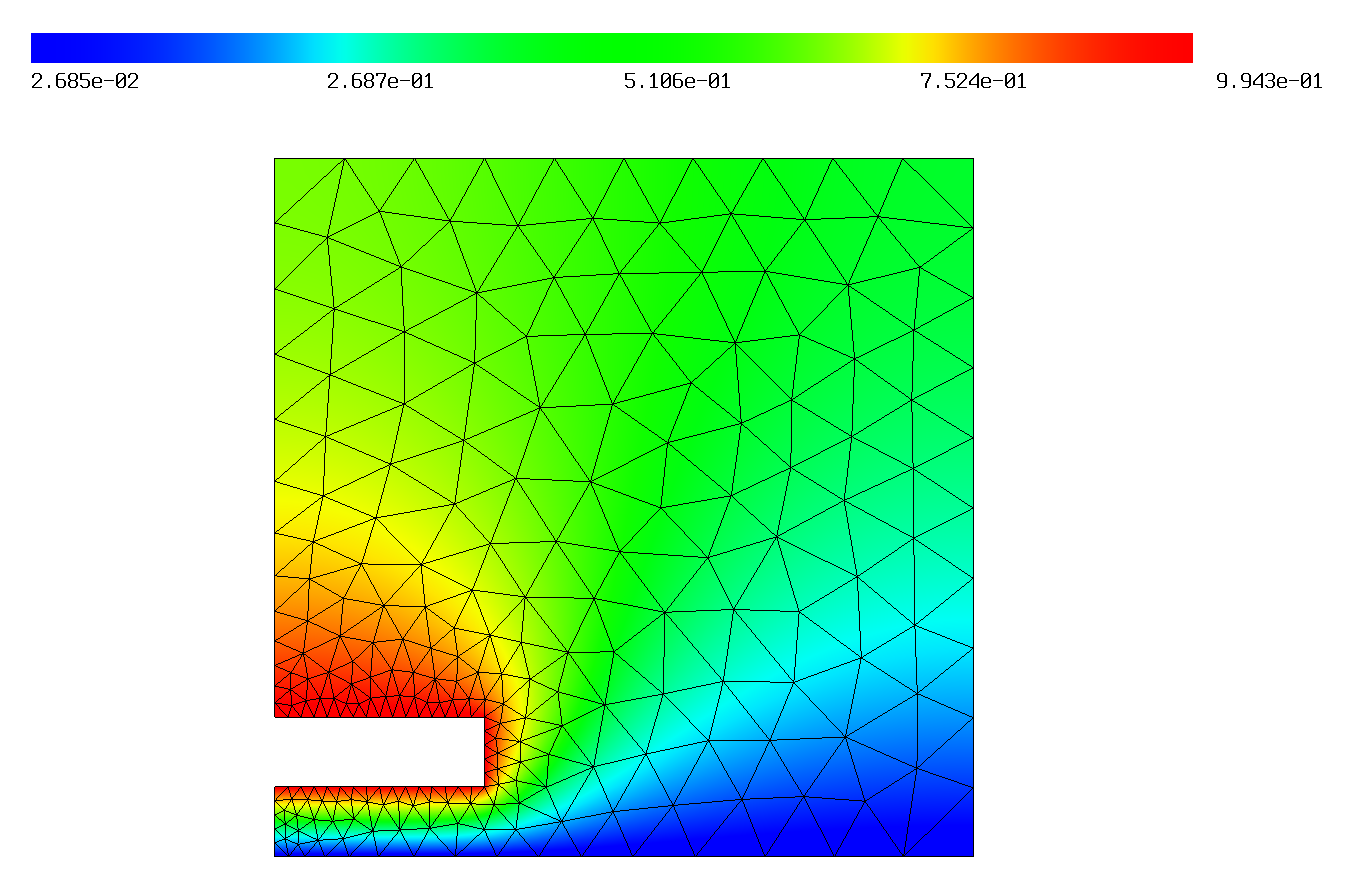
\includegraphics[width=0.7\linewidth]{../Netgen/pde1}
	\caption{Simulation eines Plattenkondesators mit Netgen}
	\label{fig:pde1}
\end{figure}

\subsection{Einfluss des fernen Randes}

Die Gr��e des berechneten Gebiets, und damit die "N�he" der Randbedingungen zueinander haben einen gro�en Einfluss auf das sich um den Kondensator ergebende Streufeld. Es wurde aus Symmetrie-Gr�nden nur der linke, obere Teil eines Kondensators in 2D berechnet.
F�r die Berechnung in Matlab wurden folgende Werte verwendet: 
\begin{itemize}
	\item $1m = 0.1 \text{Skaleneinheiten}$
	\item PDGL: $ - \nabla \cdot c \nabla u = 0$ wobei $c=1$ ist.
	\item Dirichletsche Randbedingungen an den Kondenstorfl�chen, an der horizontalen Symmetrie-Achse, sowie am fernen Rand (rechts und oben).
	\item Neumansche Randbedingung an der vertikalen Symmetrie-Achse
\end{itemize}
\textit{Info:} Aufgrund anhaltender Installatiosprobleme mit Python unter OS X wurden alle Simulationen mit dem \textit{pdetool} von Matlab gemacht. 

\begin{figure}[ht]
	\centering
\begin{tabular}{cc}
\begin{subfigure}{0.45\textwidth}
	\centering
	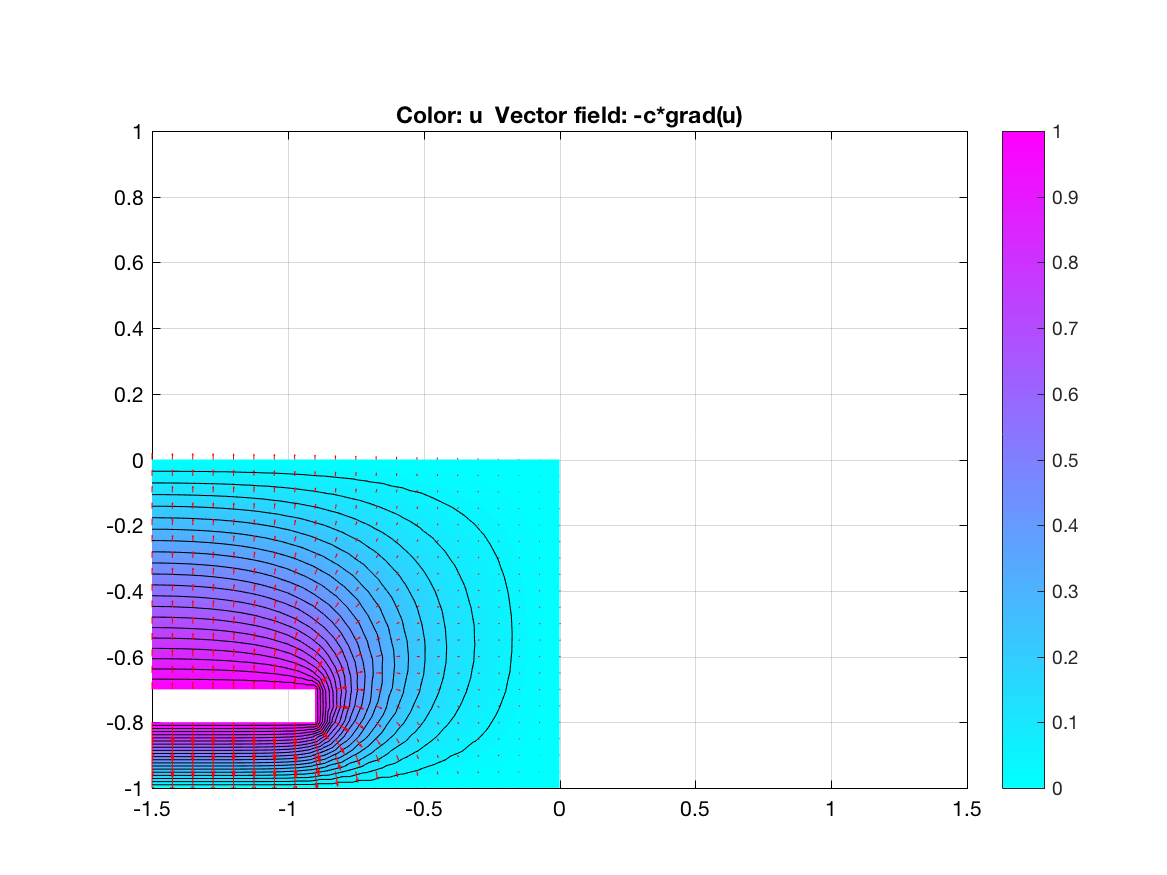
\includegraphics[width=\linewidth]{../Netgen/pdetool/pde-near}
	\caption{Rand sehr nah, 1.5 x 1}
	\label{fig:pde-near}
\end{subfigure} &
\begin{subfigure}{0.45\textwidth}
	\centering
	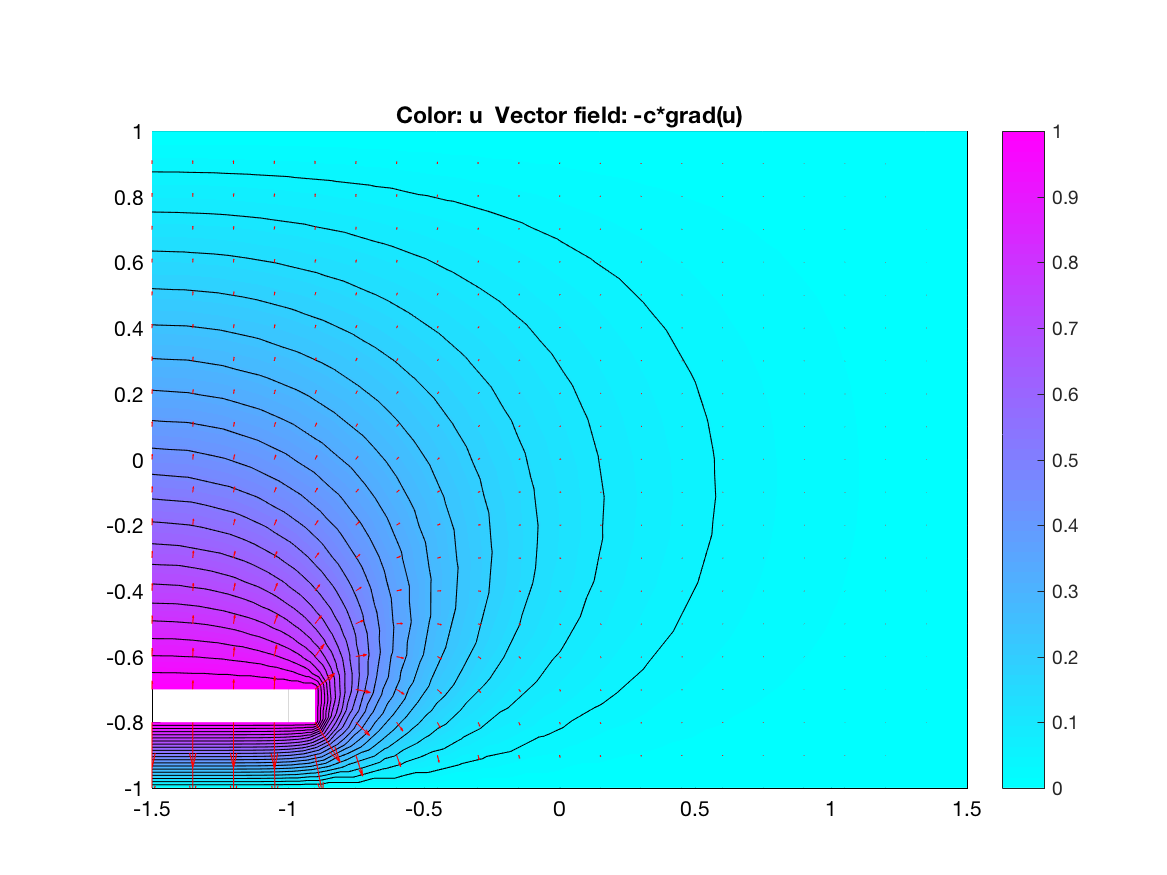
\includegraphics[width=\linewidth]{../Netgen/pdetool/pde-far}
	\caption{Rand nah, 3 x 2}
	\label{fig:pde-far}
\end{subfigure} \\
\begin{subfigure}{0.45\textwidth}
	\centering
	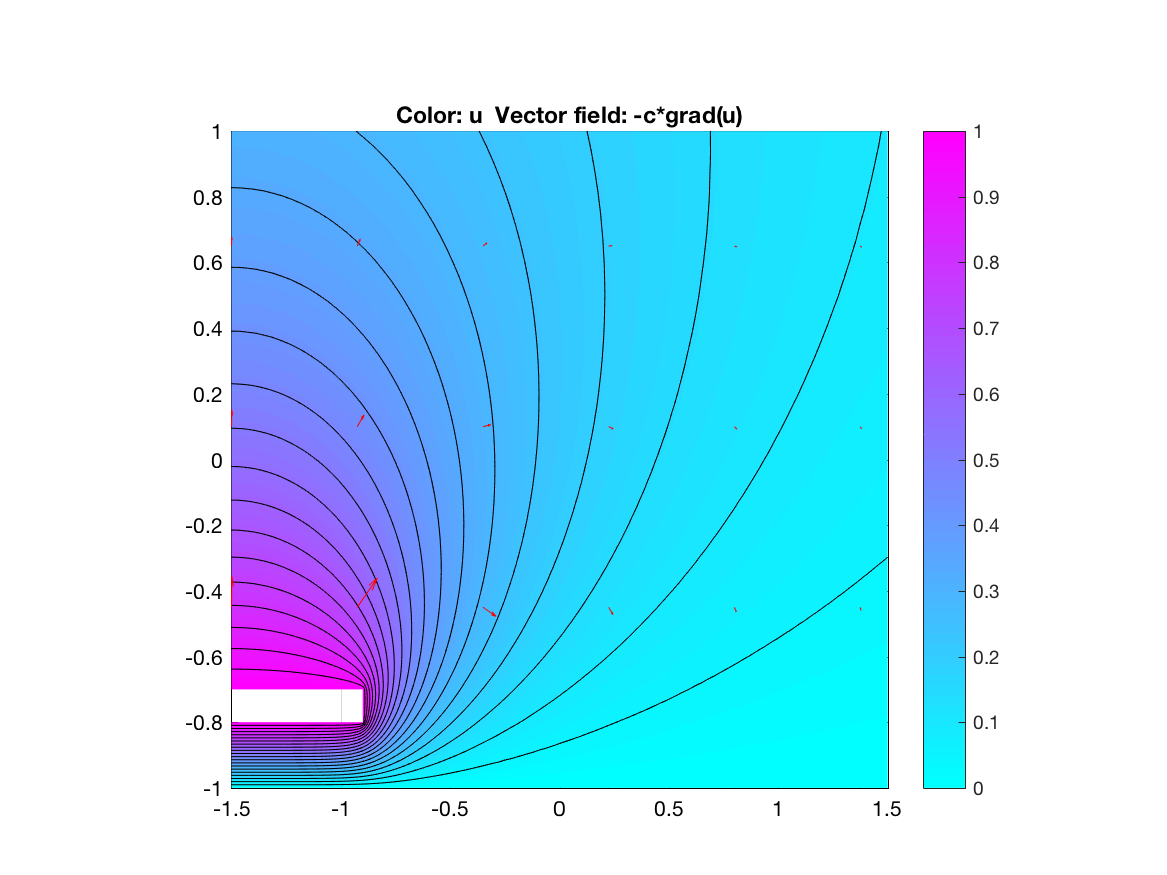
\includegraphics[width=\linewidth]{../Netgen/pdetool/pde-not-so-very-far}
	\caption{Gro�es Gebiet 10 x 10}
	\label{fig:pde-far}
\end{subfigure} &
\begin{subfigure}{0.45\textwidth}
	\centering
	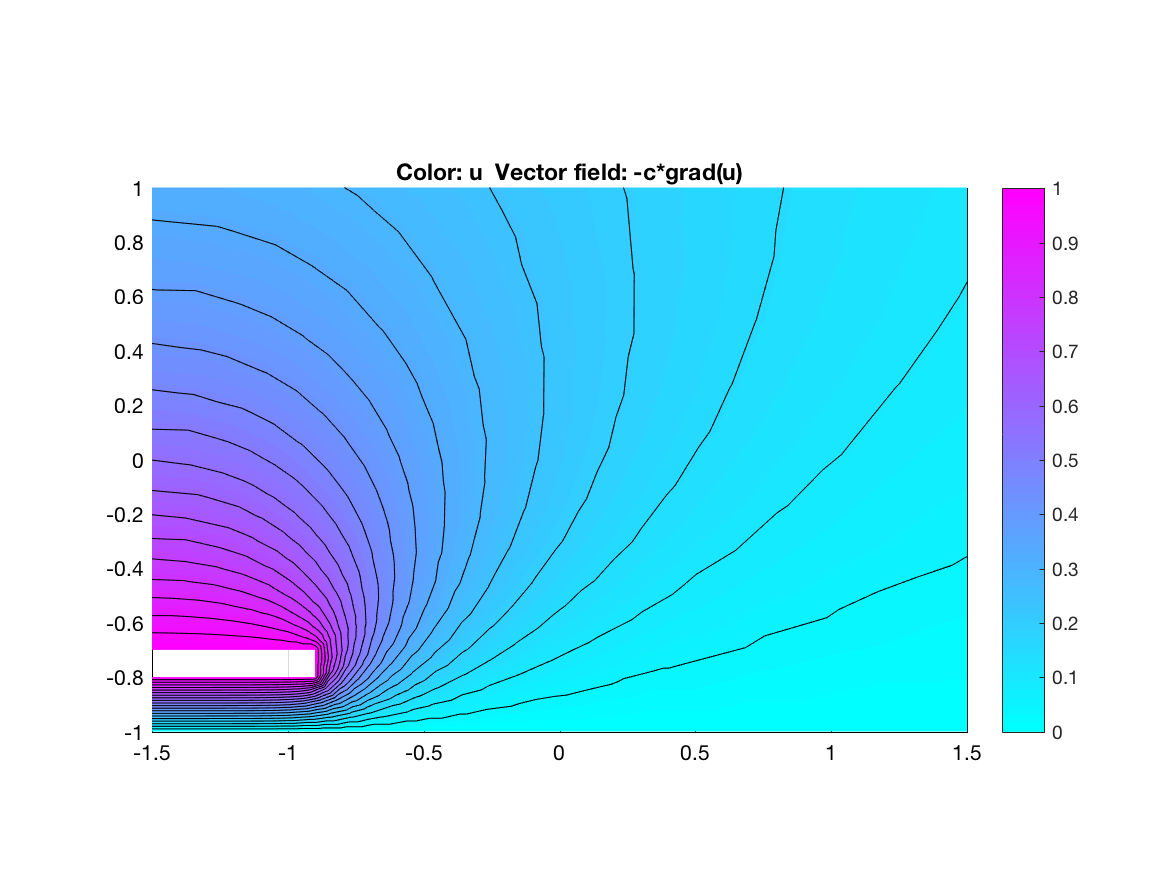
\includegraphics[width=\linewidth]{../Netgen/pdetool/pde-very-far}
	\caption{Riesen Gebiet 100 x 100}
	\label{fig:pde-far}
\end{subfigure}
\end{tabular}
\caption{Untersuchen des Einflusses des fernen Randes}
\end{figure}
	
	\appendix
	\listoffigures
	\listoftables
	

\end{document}